% file: 3-9-connectivity/menger-theorem-case-II.tex
% Based on the proof of the book ``A First Course in Graph Theory'' by Gary Chartrand and Ping Zhang
% The graph is from the book ``Introduction to Graph Theory'' by Douglas B. West.

\documentclass[tikz]{standalone}
\usetikzlibrary{positioning, shapes, fit}

\begin{document}
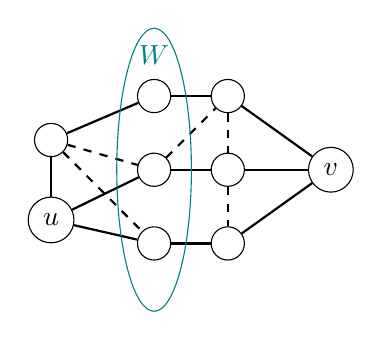
\begin{tikzpicture}[v/.style = {draw, circle, minimum size = 12pt},
  every edge/.style = {draw, thick},
  vc/.style = {draw, teal, ellipse}]
  \node (u) [v] {$u$};
  \node (ua) [v, above = 0.50cm of u] {};

  \node (w1) [v, above right = 0.25cm and 1.0cm of ua] {};
  \node (w2) [v, below = 0.50cm of w1] {};
  \node (w3) [v, below = 0.50cm of w2] {};

  \node (s1) [v, right = 0.50cm of w1] {};
  \node (s2) [v, right = 0.50cm of w2] {};
  \node (s3) [v, right = 0.50cm of w3] {};

  \node (v) [v, right = 0.80cm of s2] {$v$};

  \path (u) edge (ua)
  	    edge (w2)
  	    edge (w3)
  	(ua) edge (w1)
	     edge[dashed] (w2)
	     edge[dashed] (w3)
	(w1) edge (s1)
	(w2) edge (s2)
	     edge[dashed] (s1)
	(w3) edge (s3)
	(s1) edge[dashed] (s2)
	     edge (v)
	(s2) edge[dashed] (s3)
	     edge (v)
	(s3) edge (v);
  
  \node (w) [vc, fit = (w1) (w2) (w3), label = {[below = 3pt, teal] $W$}] {};
\end{tikzpicture}
\end{document}
